
\begin{table}[!htbp]
	\centering
	\renewcommand{\arraystretch}{1.2}
	\setlength{\tabcolsep}{0.35em}
	\resizebox{\columnwidth}{!}{%
		\begin{tabular}{@{}lcccccc@{}}
			\hline
			\textbf{Method} & \textit{Train Samples} & \textit{Lotka-V.} & \textit{Belousov-Z.} & \textit{Grey-Scott} & \textit{Multiphase} & \textit{THM} \\
			\hline
			\multirow{2}{*}{$\text{FNO}_{c}$} & 512 & 0.3251 $\pm$0.0507 & 0.0058 $\pm$1.4e-4 & 0.0056 $\pm$0.0001 & 0.0232 $\pm$0.0005 & 0.1826 $\pm$0.0088 \\
			& 1024 & 0.1499 $\pm$0.0097 & 0.0022 $\pm$4.4e-5 & 0.0042 $\pm$7.8e-5 & 0.0684 $\pm$0.1071 & 0.1577 $\pm$0.0073 \\
			\hline
			\multirow{2}{*}{CMWNO} & 512 & 0.3989 $\pm$0.0422 & 0.0375 $\pm$0.0015 & - & - & - \\
			& 1024 & 0.3876 $\pm$0.0357 & 0.0336 $\pm$0.0019 & - & - & - \\
			\hline
			\multirow{2}{*}{$\text{UFNO}_{c}$} & 512 & 0.2519 $\pm$0.0518 & 0.0239 $\pm$7.7e-4 & 0.0083 $\pm$0.0003 & 0.0241 $\pm$0.0004 & 0.1824 $\pm$0.0094 \\
			& 1024 & 0.1677 $\pm$0.0120 & 0.0122 $\pm$5.1e-4 & 0.0044 $\pm$9.8e-5 & 0.0137 $\pm$0.0010 & 0.1496 $\pm$0.0086 \\
			\hline
			\multirow{2}{*}{$\text{Transolver}_{c}$} & 512 & 0.2606 $\pm$0.0515 & 0.0329 $\pm$0.0089 & 0.0251 $\pm$0.0009 & 0.0503 $\pm$0.0311 & 0.2176 $\pm$0.0123 \\
			& 1024 & 0.1262 $\pm$0.0348 & 0.0151 $\pm$0.0023 & 0.0174 $\pm$0.0009 & 0.0185 $\pm$0.0037 & 0.1916 $\pm$0.0126 \\
			\hline
			\multirow{2}{*}{$\text{DeepONet}_{c}$} & 512 & 0.4024 $\pm$0.0143 & 0.6491 $\pm$0.0199 & 0.7655 $\pm$0.0039 & 0.1123 $\pm$0.0051 & 0.2867 $\pm$0.0199 \\
			& 1024 & 0.3005 $\pm$0.0285 & 0.5810 $\pm$0.0352 & 0.6700 $\pm$0.0240 & 0.0766 $\pm$0.0049 & 0.2388 $\pm$0.0125 \\
			\hline
			\multirow{2}{*}{\ours-RNN} & 512 & 0.0920 $\pm$0.0085 & 0.0033 $\pm$2.6e-4 & 0.0062 $\pm$0.0039 & 0.0225 $\pm$0.0108 & \textbf{0.1607 $\pm$0.0089} \\
			& 1024 & 0.0531 $\pm$0.0100 & 0.0015 $\pm$9.7e-5 & 0.0035 $\pm$8.0e-5 & 0.0110 $\pm$0.0010 & \textbf{0.1407 $\pm$0.0097} \\
			\hline
			\multirow{2}{*}{\ours-ATN} & 512 & \textbf{0.0918 $\pm$0.0042} & \textbf{0.0016 $\pm$2.7e-5} & \textbf{0.0050 $\pm$0.0016} & \textbf{0.0182 $\pm$0.0011} & 0.1647 $\pm$0.0092 \\
			& 1024 & \textbf{0.0510 $\pm$0.0048} & \textbf{0.0008 $\pm$2.6e-5} & \textbf{0.0035 $\pm$7.2e-5} & \textbf{0.0110 $\pm$0.0009} & 0.1442 $\pm$0.0066 \\
			\hline
	\end{tabular}}
	\vspace{1em}
	\caption{\small Comparison of relative $L_2$ prediction errors (mean $\pm$ standard deviation over 5-runs) for COMPOL variants (COMPOL-RNN, COMPOL-ATN) against baseline neural operators (FNO, UFNO, Transolver, DeepONet, CMWNO) across five multi-physics benchmark datasets, evaluated with 512 and 1024 training samples. Bold values indicate the best performance for each case.}
	\label{tab:nrmse}
\end{table}

\section{Experiment}
%\vnegxxs
\paragraph{Benchmarks} We evaluated our framework’s performance on predicting solutions for coupled multi-physics PDE systems using five benchmark test cases: 1-D Lotka-Volterra equations~\citep{murray2007mathematical} (2 processes), 1-D Belousov-Zhabotinsky equations~\citep{petrov1993controlling} (3 processes), 2-D Gray-Scott equations~\citep{pearson1993complex} (2 processes), 2-D multiphase flow of oil and water in geological storage~\citep{bear2010modeling,hashemi2021pore,abou2013petroleum} (2 processes), and a 2-D Thermal-Hydro-Mechanical problem ~\cite{gao2020three}(5 processes considering strain components separately). These diverse equations represent broad scientific and engineering applications. Detailed descriptions of these benchmarks are provided in the Appendix \ref{sec:appx-synt}, \ref{sec:appx-mf} and \ref{sec:appx-thm} Training datasets were generated with numerical solvers using 256-point meshes for 1-D cases and 64×64 meshes for 2-D cases. We trained models on two dataset sizes (512 and 1024 samples) and evaluated performance on an independent test set of 200 examples. Coefficients and boundary conditions remained constant to isolate effects of varying initial conditions. The primary objective was to assess our framework’s capability to map initial conditions ($t=0$) to final solution fields ($t=T$), highlighting its ability to model complex interactions and dynamics.
%\vnegxxs
\paragraph{Competing Methods} To evaluate our proposed coupled multi-physics neural operator framework, we compare two variants—\ours-RNN (recurrent aggregation) and \ours-ATN (attention-based aggregation)—against state-of-the-art neural operators: FNO ~\citep{li2020fourier}, UFNO~\citep{wen2022u}, Transolver~\citep{wu2024transolver}, DeepONet~\cite{lu2021learning}, and CMWNO~\citep{xiao2023coupled}, each using their official implementations. Except for CMWNO, these baselines are not inherently designed for multi-physics modeling. Therefore, we adapt them by concatenating process inputs and outputs across their respective channels (e.g., FNO\textsubscript{c}). For consistency, all models were implemented in PyTorch~\citep{paszke2019pytorch} and trained with the Adam optimizer~\citep{diederik2014adam} (learning rate = 0.001). Except for CMWNO, which employed a step scheduler (as in its original implementation), all models used a cosine annealing schedule~\citep{loshchilov2016sgdr}. Models were trained for 500 epochs, sufficient for convergence in all cases except DeepONet, which required 10,000 epochs. Experiments were conducted on NVIDIA A100 GPUs. Robustness was ensured via 5-fold cross-validation, with performance evaluated using average relative $L_2$ error and corresponding standard deviations across folds. Due to implementation constraints, CMWNO experiments were limited to 1-D scenarios.

\begin{figure*}[!htbp]
	\centering
	\setlength\tabcolsep{0.01pt}
	\captionsetup[subfigure]{aboveskip=0pt,belowskip=0pt}
	\begin{tabular}[c]{c}
		\begin{subfigure}[t]{0.8\textwidth}
			\centering
			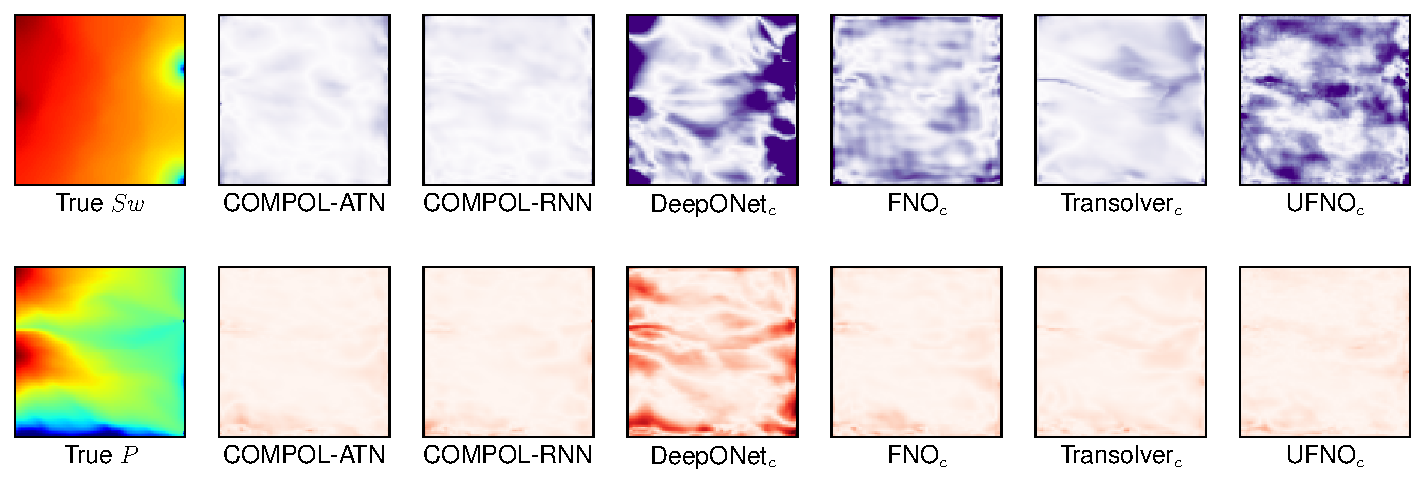
\includegraphics[width=\textwidth]{./figs/mf-new/errors_MF_id23.pdf}
		\end{subfigure} 
		\\
		\begin{subfigure}[t]{0.8\textwidth}
			\centering
			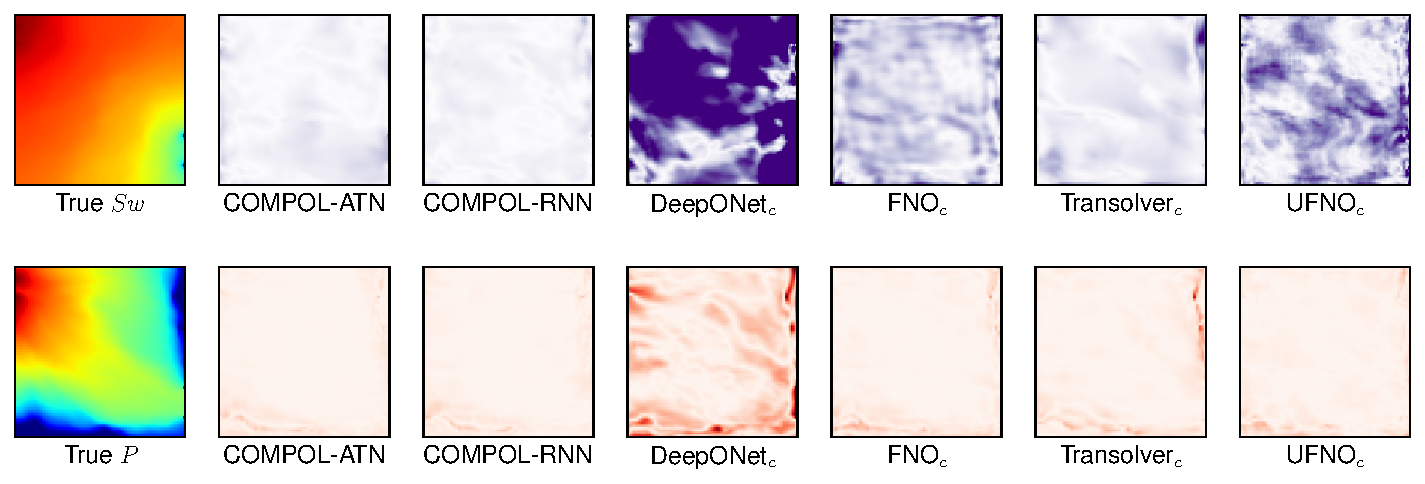
\includegraphics[width=\textwidth]{./figs/mf-new/errors_MF_id3.pdf}
		\end{subfigure} 
	\end{tabular}
	\caption{\small Element-wise solution error of coupled multiphase flow. The left most column is the ground-truth phase pressure $P$ and saturation $S_w$. The other columns are the absolute errors of each method. The lighter the color, the smaller the error.} 	
	\label{fig:vis_errs_mf}
\end{figure*}
%\vnegxs
\subsection{Analysis of Predictive Performance}
%\vnegxs
The experimental results in Table \ref{tab:nrmse} present the predictive performance of COMPOL-RNN (recurrent aggregation) and COMPOL-ATN (attention-based aggregation) compared to baseline neural operators (FNO, UFNO, Transolver, DeepONet, and CMWNO), evaluated separately for 512 and 1024 training samples.For 512 training samples, COMPOL-ATN consistently achieves the lowest prediction errors, outperforming baseline methods with improvements up to 72.41\%. COMPOL-RNN also demonstrates strong performance, showing improvements up to 63.48\%, though slightly underperforming on the Grey-Scott dataset. When increasing the training set size to 1024 samples, COMPOL-ATN maintains superior performance, achieving improvements up to 63.64\% compared to baselines, notably excelling in Lotka-Volterra and Belousov-Zhabotinsky datasets. COMPOL-RNN also continues robust performance with improvements up to 57.92\% across benchmarks. Baseline neural operators adapted for multi-physics tasks exhibit significantly higher errors at both training scales. CMWNO, despite being explicitly designed for multi-physics modeling, consistently underperforms relative to both COMPOL variants.These results affirm the superior effectiveness and scalability of COMPOL methods in multi-physics modeling scenarios. We also provide a visualization of the element-wise errors for the 2-D multiphase flow in Figure \ref{fig:vis_errs_mf}, along with a comparative visualization of predictions for the 1-D benchmarks in Section \ref{sec:pred_ground}.


\subsection{Ablation Study of Coupling Mechanisms}
%\vnegxs
To elucidate the factors underlying COMPOL’s superior performance, we dissect its coupling mechanism into three core components: feature aggregation ($a_{l-1}$), augmentation ($b_{l-1}$), and mixing ($c_{l-1}$), as depicted in Figure \ref{fig:model}. A detailed evaluation of each component's impact is provided in the Appendix \ref{sec:appx-coupling}. Here, we address two crucial questions.

\begin{table*}[!htbp]
	\setlength{\tabcolsep}{0.9em} % Adjust column spacing for better readability
	\renewcommand{\arraystretch}{1.1} % Adjust row spacing
	\centering
	\resizebox{\columnwidth}{!}{%
		\begin{tabular}{@{}lcccccc@{}}
			\hline
			\textbf{Method} & \textit{Modes} & \textit{Width} & \textit{Layers} & \textit{Params Count (M)} & \textit{BZ} & \textit{LV} \\
			\hline
			$\text{FNO}_{\textit{c}} \ \text{(default)}$ & $16$ & $64$ & $4$ & $0.5832$ & $0.0022 \pm 4.4\text{e-5}$ & $0.1499 \pm 0.0097$ \\
			
			$\text{FNO}_{\textit{c}} $ & $96$ & $64$ & $4$ & $3.2047$ & $ 0.0018 \pm 4.9\text{e-5}$ & $0.1183 \pm 0.0106$ \\
			
			$\text{FNO}_{\textit{c}}  $ & $64$ & $64$ & $6$ & $3.2296$ & $ 0.0020 \pm 4.4\text{e-5}$ & $0.1303 \pm 0.0152$ \\
			
			$\text{FNO}_{\textit{c}}$ & $48$ & $64$ & $8$ & $3.2546$ & $0.0032 \pm 0.0001$ & $0.1488 \pm 0.0160$ \\
			
			$\text{FNO}_{\textit{c}} $ & $16$ & $224$ & $2$ & $3.6169$ & $0.0014 \pm 2.6\text{e-5}$ & $0.1757 \pm 0.0102$ \\
			
			$\text{FNO}_{\textit{c}} $ & $16$ & $128$ & $6$ & $3.4774$ & $0.0018 \pm 3.8\text{e-5}$ & $0.1761 \pm 0.0099$ \\
			
			$\text{FNO}_{\textit{c}} $ & $16$ & $160$ & $4$ & $3.6392$ & $0.0016 \pm 4\text{e-5}$ & $0.1698 \pm 0.0090$ \\
			
			\ours-RNN & $16$  & $64$ & $4$ & \shortstack{{BZ: $3.0749$ } \\ {LV: $2.4880$}} & $0.0015 \pm 9.7\text{e-5}$  & $ 0.0531 \pm 0.0100$ \\
			
			\ours-ATN & $16$  & $64$ & $4$ & \shortstack{{BZ: $2.1029$} \\ {LV: $1.4925$}} & $\mathbf{0.0008 \pm 2.6\text{e-5}}$  & $\mathbf{0.0510 \pm 0.0048}$ \\
			\hline
		\end{tabular}
	}
	\caption{\small Comparison of testing relative $L_2$ errors for FNO variants expanded to match COMPOL’s parameter count versus \ours-RNN and \ours-ATN, evaluated on Belousov–Zhabotinsky (BZ) and Lotka–Volterra (LV) equations. Results show that COMPOL’s superior performance is primarily due to its coupling mechanism rather than merely increased parameters.}
	\label{tab:ablation_params}
\end{table*}

%\begin{wraptable}{r}{0.5\textwidth}
%	\setlength{\intextsep}{1pt}% Reduce vertical spacing above/below
%	\setlength{\columnsep}{5pt}% Reduce horizontal spacing
%	\centering
%	\renewcommand{\arraystretch}{1.0}
%	\setlength{\tabcolsep}{0.2em}
%	{\small
%		\begin{tabular}{@{}lcc@{}}
%			\hline
%			\textbf{Method} & \textit{ntrain=512} & \textit{ntrain=1024} \\
%			\hline
%			$\text{FNO}$ & $0.0715 \pm 0.0033$ & $0.0422 \pm 0.0037$ \\
%			CMWNO & $0.4441 \pm 0.0134$ & $0.4509 \pm 0.0168$ \\
%			$\text{UFNO}$ & $0.1043 \pm 0.0061$ & $0.0565 \pm 0.0012$ \\
%			$\text{Transolver}$ & $0.1264 \pm 0.0733$ & $0.4066 \pm 0.4248$ \\
%			$\text{DeepONet}$ & $0.4007 \pm 0.0216$ & $0.3749 \pm 0.0181$ \\
%			\ours-RNN & $0.0397 \pm 0.0030$ & $0.0197 \pm 0.0013$ \\
%			\ours-ATN & $\mathbf{0.0200 \pm 0.0021}$ & $\mathbf{0.0106 \pm 0.0006}$ \\
%			\hline
%	\end{tabular}}
%	\caption{\small Comparison of prediction accuracy (relative $L_2$ error) for the single-process Burgers' equation across methods trained with 512 and 1024 examples. Results averaged over 5 runs (500 epochs each), highlighting superior performance of \ours with latent aggregation.}
%	\label{tab:ablation_single}
%\end{wraptable}
%\vnegxxs

\begin{table}[!htbp]
	\setlength{\intextsep}{1pt}% Reduce vertical spacing above/below
	\setlength{\columnsep}{5pt}% Reduce horizontal spacing
	\centering
	\renewcommand{\arraystretch}{1.0}
	\setlength{\tabcolsep}{0.2em}
	{\small
		\begin{tabular}{@{}lcc@{}}
			\hline
			\textbf{Method} & \textit{ntrain=512} & \textit{ntrain=1024} \\
			\hline
			$\text{FNO}$ & $0.0715 \pm 0.0033$ & $0.0422 \pm 0.0037$ \\
			CMWNO & $0.4441 \pm 0.0134$ & $0.4509 \pm 0.0168$ \\
			$\text{UFNO}$ & $0.1043 \pm 0.0061$ & $0.0565 \pm 0.0012$ \\
			$\text{Transolver}$ & $0.1264 \pm 0.0733$ & $0.4066 \pm 0.4248$ \\
			$\text{DeepONet}$ & $0.4007 \pm 0.0216$ & $0.3749 \pm 0.0181$ \\
			\ours-RNN & $0.0397 \pm 0.0030$ & $0.0197 \pm 0.0013$ \\
			\ours-ATN & $\mathbf{0.0200 \pm 0.0021}$ & $\mathbf{0.0106 \pm 0.0006}$ \\
			\hline
	\end{tabular}}
	\caption{\small Comparison of prediction accuracy (relative $L_2$ error) for the single-process Burgers' equation across methods trained with 512 and 1024 examples. Results averaged over 5 runs (500 epochs each), highlighting superior performance of \ours with latent aggregation.}
	\label{tab:ablation_single}
\end{table}

\paragraph{Increasing Native FNO to Match Parameter Count}
COMPOL employs separate neural operators for each physical process in a multi-physics system and integrates an aggregation mechanism for inter-process information exchange in latent space. Consequently, COMPOL inherently has at least $M$ times more parameters than a single FNO using naive concatenation, where $M$ is the number of coupled processes. This raises the question: does COMPOL's superior performance primarily stem from having more parameters? To investigate this, we increased the Fourier modes, network width, and layers of the FNO to match COMPOL's parameter count. Evaluations on the Belousov-Zhabotinsky (BZ, 3 processes) and Lotka-Volterra (LV, 2 processes) equations using 1024 samples, and present the relative $L_2$ errors in Table \ref{tab:ablation_params}. The results indicate that while expanding the FNO parameter count does yield performance improvements, further increasing width or layers does not significantly reduce predictive errors. Thus, the superiority of COMPOL is not merely due to higher parameter counts but is largely attributable to its effective and scalable coupling mechanism.
%\vnegxxs
\paragraph{Improvement over Single-Process Simulations}
We further examine whether COMPOL’s latent aggregation mechanisms can enhance predictive performance for single-process simulations. Specifically, we evaluate COMPOL on the single-process Burgers’ equation using training sets of 512 and 1024 examples, comparing results against baseline methods (Table \ref{tab:ablation_single}). Results show that COMPOL significantly improves predictive accuracy, even in single-process scenarios, by effectively leveraging advanced latent aggregation techniques (attention-based and recurrent methods). These mechanisms enrich latent feature representations, implicitly regularize learning, adaptively select relevant features, and better capture underlying temporal dynamics. Consequently, COMPOL demonstrates improved optimization stability, superior generalization, and increased overall accuracy.








